\section{Experiments: drift, optimizers, and the saddle}\label{sec:part2-exp}

\subsection{E10: what happens to a legible code}
Starting from a legible code with $d=32$ features in $n=16$ coordinates, we continue training under Adam in four
ways (\cref{tab:e10}, \cref{fig:e10}).
\begin{table}[h]\centering\footnotesize
\resizebox{\linewidth}{!}{\begin{tabular}{@{}l ccccc@{}}\toprule
condition (after 6000 steps) & receiver F1 & frozen & recalibrated & refit & neurons/feature \\\midrule
legible checkpoint & 0.915\,$\pm$\,0.018 & 0.922\,$\pm$\,0.019 & 0.927\,$\pm$\,0.015 & 0.922\,$\pm$\,0.017 & 1.159\,$\pm$\,0.123 \\\midrule
release & 0.984\,$\pm$\,0.001 & 0.714\,$\pm$\,0.047 & 0.865\,$\pm$\,0.061 & 0.937\,$\pm$\,0.013 & 1.733\,$\pm$\,0.336 \\
pressure & 0.922\,$\pm$\,0.006 & 0.790\,$\pm$\,0.066 & 0.839\,$\pm$\,0.053 & 0.893\,$\pm$\,0.015 & 1.085\,$\pm$\,0.055 \\
pressure+budget & 0.827\,$\pm$\,0.012 & 0.772\,$\pm$\,0.052 & 0.798\,$\pm$\,0.026 & 0.822\,$\pm$\,0.021 & 1.214\,$\pm$\,0.216 \\
pressure+monitor & 0.907\,$\pm$\,0.004 & 0.803\,$\pm$\,0.018 & 0.872\,$\pm$\,0.030 & 0.870\,$\pm$\,0.011 & 1.241\,$\pm$\,0.156 \\
\bottomrule\end{tabular}}
\caption{E10: four continuations of a legible code ($d=32$, $n=16$, Adam), mean $\pm$ sd over 5 seeds. ``pressure'':
feature density $p$ raised from 0.1 to 0.3; ``budget'': the $\ell_1$ legibility budget is kept; ``monitor'': the
frozen monitor's loss is added to the training loss. Receiver$-$refit gap: 0.029\,$\pm$\,0.019 under pressure, 0.037\,$\pm$\,0.011 with the monitor in the loss.}
\label{tab:e10}\end{table}

\begin{figure}[h]
\centering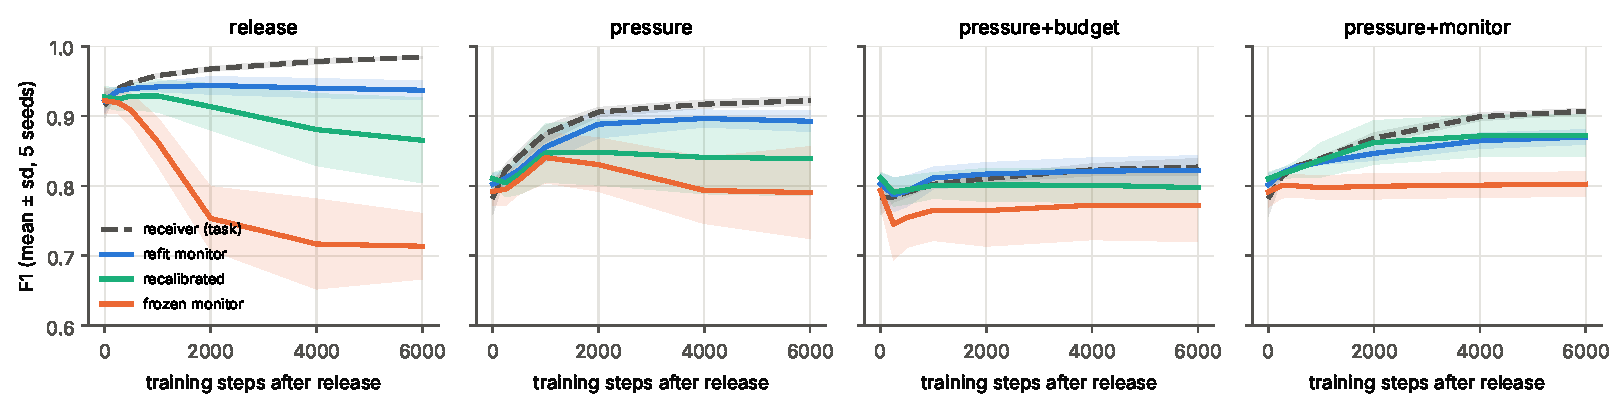
\includegraphics[width=\linewidth]{figs/e10_drift.pdf}
\caption{E10: the four readings of \cref{fig:ladder} over training, mean $\pm$ sd over 5 seeds.}
\label{fig:e10}
\end{figure}

\emph{Release} (the budget is removed and nothing else changes) is the cleanest case. The code spreads: neurons per
feature rise from $1.16$ to $1.73$. The frozen monitor falls from $0.92$ to $0.71$. But a per-feature recalibration
of scale and bias recovers most of that ($0.87$), and a refit monitor reads the new code as well as the old ($0.94$).
The honest decomposition of the frozen monitor's loss is roughly two-thirds calibration and one-third direction.
Neither is invisible: a monitor that is refit, or even just recalibrated, on fresh labelled data sees through it.

\emph{Pressure} (three times as many active features) does not spread the code at the feature level; neurons per
feature fall slightly. \emph{Pressure with the budget kept} holds the code legible at a visible price in task
performance (receiver F1 $0.83$ against $0.92$): the legibility tax. \emph{Pressure with the frozen monitor in the
loss} does what one would expect of a training signal: the frozen monitor's score stops falling. The worry from
earlier drafts was that the receiver would meanwhile build a channel no monitor can read. At this scale we see no
sign of it: the receiver$-$refit gap is the same with and without the monitor in the loss, within seed-to-seed
variation.

\subsection{E11: the update rule}
We now hold the task fixed, remove the budget, and change only the update rule (\cref{tab:e11},
\cref{fig:e11}).
\begin{table}[h]\centering\footnotesize\setlength{\tabcolsep}{3pt}
\resizebox{\linewidth}{!}{\begin{tabular}{@{}l cccccc@{}}\toprule
optimizer (6000 steps, budget removed) & receiver F1 & frozen & recalibrated & refit & neurons/feature & leak \\\midrule
$d=12$, legible start & 0.985\,$\pm$\,0.003 & 0.998\,$\pm$\,0.004 & 0.998\,$\pm$\,0.004 & 0.998\,$\pm$\,0.004 & 1.033\,$\pm$\,0.066 & 0.013\,$\pm$\,0.026 \\
\quad Adam & 1.000\,$\pm$\,0.000 & 0.998\,$\pm$\,0.004 & 0.998\,$\pm$\,0.004 & 1.000\,$\pm$\,0.000 & 2.066\,$\pm$\,0.097 & 0.330\,$\pm$\,0.016 \\
\quad SGD & 1.000\,$\pm$\,0.000 & 0.998\,$\pm$\,0.003 & 0.998\,$\pm$\,0.003 & 1.000\,$\pm$\,0.000 & 1.107\,$\pm$\,0.132 & 0.045\,$\pm$\,0.052 \\
\quad hybrid: SGD sender, Adam receiver & 1.000\,$\pm$\,0.000 & 0.998\,$\pm$\,0.003 & 0.998\,$\pm$\,0.003 & 1.000\,$\pm$\,0.000 & 1.078\,$\pm$\,0.094 & 0.032\,$\pm$\,0.038 \\
\quad reverse: Adam sender, SGD receiver & 1.000\,$\pm$\,0.000 & 0.998\,$\pm$\,0.004 & 0.998\,$\pm$\,0.004 & 1.000\,$\pm$\,0.000 & 1.726\,$\pm$\,0.215 & 0.315\,$\pm$\,0.172 \\
\quad SGD, large step & 0.856\,$\pm$\,0.201 & 0.430\,$\pm$\,0.142 & 0.516\,$\pm$\,0.202 & 0.843\,$\pm$\,0.211 & 3.884\,$\pm$\,0.545 & 0.620\,$\pm$\,0.164 \\
\midrule
$d=32$, legible start & 0.916\,$\pm$\,0.017 & 0.927\,$\pm$\,0.022 & 0.934\,$\pm$\,0.020 & 0.926\,$\pm$\,0.021 & 1.269\,$\pm$\,0.172 & 0.071\,$\pm$\,0.028 \\
\quad Adam & 0.982\,$\pm$\,0.002 & 0.708\,$\pm$\,0.052 & 0.867\,$\pm$\,0.070 & 0.941\,$\pm$\,0.015 & 1.775\,$\pm$\,0.432 & 0.069\,$\pm$\,0.030 \\
\quad SGD & 0.960\,$\pm$\,0.004 & 0.796\,$\pm$\,0.083 & 0.919\,$\pm$\,0.039 & 0.943\,$\pm$\,0.014 & 1.561\,$\pm$\,0.350 & 0.102\,$\pm$\,0.048 \\
\quad hybrid: SGD sender, Adam receiver & 0.982\,$\pm$\,0.002 & 0.760\,$\pm$\,0.050 & 0.886\,$\pm$\,0.055 & 0.944\,$\pm$\,0.015 & 1.765\,$\pm$\,0.401 & 0.098\,$\pm$\,0.037 \\
\quad reverse: Adam sender, SGD receiver & 0.962\,$\pm$\,0.003 & 0.769\,$\pm$\,0.081 & 0.916\,$\pm$\,0.040 & 0.944\,$\pm$\,0.013 & 1.547\,$\pm$\,0.367 & 0.065\,$\pm$\,0.033 \\
\quad SGD, large step & 0.426\,$\pm$\,0.357 & 0.232\,$\pm$\,0.045 & 0.143\,$\pm$\,0.195 & 0.426\,$\pm$\,0.301 & 2.361\,$\pm$\,0.842 & 0.687\,$\pm$\,0.208 \\
\bottomrule\end{tabular}}
\caption{E11: same task, legibility budget removed, five update rules; mean $\pm$ sd over 5 seeds. Learning rates:
Adam $3\times10^{-3}$, SGD $0.05$, large-step SGD $0.5$. ``leak'': fraction of sender weight energy outside each
feature's legible coordinate. $d=12<n$: empty coordinates exist; $d=32>n$: superposition.}
\label{tab:e11}\end{table}

\begin{figure}[h]
\centering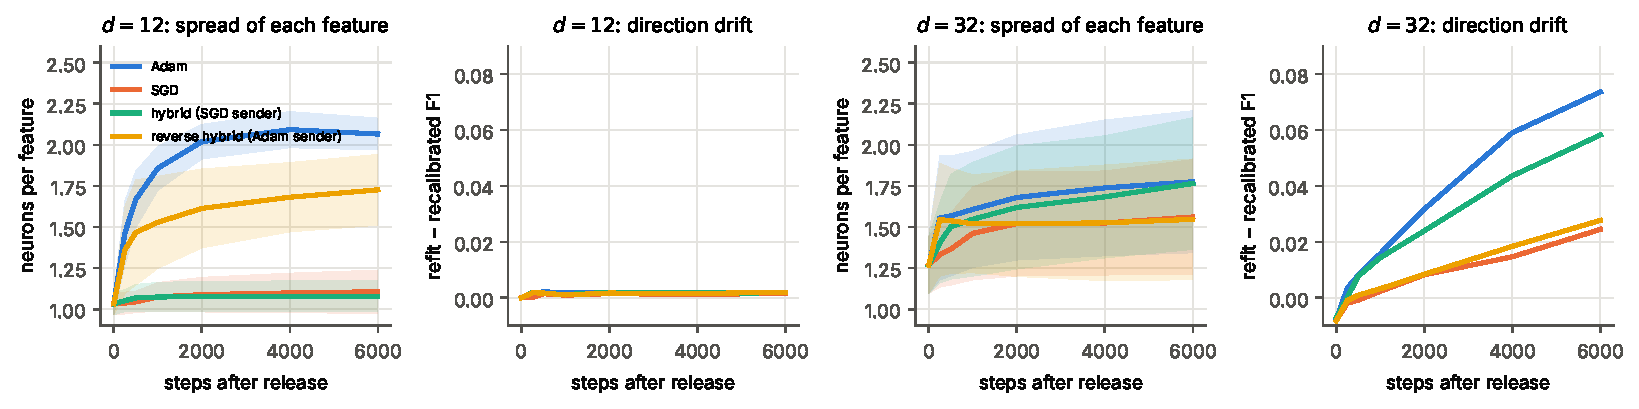
\includegraphics[width=\linewidth]{figs/e11_optimizers.pdf}
\caption{E11: feature spread and direction drift (refit minus recalibrated F1) after the budget is removed, for four
update rules, mean $\pm$ sd over 5 seeds. Large-step SGD diverges on some seeds and is shown only in \cref{tab:e11}.}
\label{fig:e11}
\end{figure}

\emph{With spare public coordinates ($d=12<n$), \cref{pred:writer} holds.} At identical task performance (F1 $1.000$
for all four rules), the sender's update rule decides whether features stay on their coordinates. Adam on the sender
spreads each feature over about two neurons, whether the receiver uses Adam ($2.07$) or SGD ($1.73$). SGD on the
sender keeps it on one ($1.11$ with SGD everywhere, $1.08$ for the hybrid with an Adam receiver). This is the
hybrid optimizer of earlier drafts, and in this regime it works as advertised. The spread is also exactly the kind
predicted by \cref{sec:saddle}: under Adam on the sender, the message densifies even when the receiver (on SGD) is
too slow to make use of it. In this regime the spread does not hurt linear monitors, which remain at $0.998$ in
every column: the new copies are redundant, and the original coordinate still carries each feature.

\emph{In superposition ($d=32>n$), \cref{pred:writer} fails.} E11's starting codes differ in how they are packed
(\file{e11\_packing.py}): at $d=12$, 11 or 12 of the 16 coordinates are used and at most one is shared; at $d=32$,
10 to 16 coordinates are shared by 2--4 features each, and at most two are empty. So \cref{lem:stationary} has
almost nothing to protect, and E15 below shows that leaks into occupied coordinates feel first-order forces. Spread and direction
drift now track the \emph{receiver's} update rule: with an Adam receiver (Adam everywhere, or the hybrid) neurons per
feature reach $1.77$ and direction drift is $0.06$--$0.07$; with an SGD receiver (SGD everywhere, or the reverse
hybrid) they are $1.55$ and $0.02$--$0.03$. These are also the configurations whose receivers learn more (task F1
$0.982$ against $0.960$). The natural reading is that, in superposition, drift away from the public frame is
a first-order response to a receiver that is still improving, and the optimizer matters through how fast the
receiver improves rather than through the sender's normalization. The hybrid optimizer does not preserve legibility
here at matched task performance.

\subsection{E15: superposition removes the critical point}
Is the legible code a critical point when coordinates are shared? We take E11's starting codes (same seeds, same
ReLU receiver), restrict each feature to its strongest coordinate while keeping whatever sharing the code had, polish
all parameters within that support on a full batch, and then measure the gradient in the directions that leave it
(\cref{tab:e15}).
\begin{table}[h]\centering\footnotesize\setlength{\tabcolsep}{3pt}
\resizebox{\linewidth}{!}{\begin{tabular}{@{}rr cc cc cc c@{}}\toprule
 & & \multicolumn{2}{c}{coordinates (of 16)} & \multicolumn{2}{c}{gradient within support} & \multicolumn{2}{c}{gradient, leaks into occupied} & leaks into \\\cmidrule(lr){3-4}\cmidrule(lr){5-6}\cmidrule(lr){7-8}
$d$ & seeds & empty & shared & norm & per entry & norm & per entry & empty, norm \\\midrule
12 & 3 & 4.3 & 0.3 & 1.9e-09--2.7e-07 & 4.3e-11--6.1e-09 & 7.7e-10--6.6e-07 & 6.4e-11--5.7e-08 & 2.7e-10--2.7e-07 \\
32 & 3 & 0.3 & 13.7 & 2.9e-02--4.1e-02 & 5.1e-04--7.3e-04 & 1.5e-01--1.8e-01 & 7.0e-03--8.1e-03 & 0.0e+00--3.9e-04 \\
\bottomrule\end{tabular}}
\caption{E15: is the legible code a critical point? Starting from E11's legible codes (same seeds, ReLU receiver), each
feature is restricted to its strongest coordinate (shared coordinates kept) and all parameters are polished within that
support (full batch of 6144, $\sigma=0.1$). Gradient norms, and root-mean-square per entry, in three groups of
directions; ranges are over seeds.}
\label{tab:e15}\end{table}

At $d=12$ the polish converges, and the legible code is a critical point in every direction, leaks included:
all gradient norms lie between $10^{-9}$ and $10^{-6}$. At $d=32$ it is not. After the same 11{,}000 full-batch steps the gradient
within the legible support is still $3$--$4\times10^{-2}$, and the gradient for leaks into occupied coordinates is
$0.15$--$0.18$ in norm, 11--14 times larger per entry. In superposition the legible support is not where the loss
wants to be. Drift away from it is a first-order response, which any optimizer will follow, and which makes the
update rule matter mainly through how fast the receiver keeps improving. That is the pattern E11 shows.

\subsection{E13: how flat is the legible critical point?}
To look for the saddle of \cref{sec:saddle} directly we use $d=12$ features (so empty coordinates exist), a smooth
softplus receiver (so second derivatives exist), and channel noise from the operating value $\sigma=0.1$ up to
$\sigma=0.9$. We match each feature to its own coordinate, restrict the sender to that legible support, and polish
everything to a critical point within it, on a fixed batch of 6144 samples. We then compute the global smallest
Hessian eigenvalue by Lanczos and, for the least saturated empty coordinate, the leak/read block of each feature
(\cref{tab:e13}, \cref{fig:e13}).
\begin{table}[h]\centering\footnotesize\setlength{\tabcolsep}{3pt}
\resizebox{\linewidth}{!}{\begin{tabular}{@{}c c cc cc cc ccc@{}}\toprule
 & sender & \multicolumn{2}{c}{residual error $\mmse$} & \multicolumn{2}{c}{gradient norm} & \multicolumn{2}{c}{global $\lambda_{\min}$} & \multicolumn{3}{c}{leak into empty coordinate (median over features)} \\\cmidrule(lr){3-4}\cmidrule(lr){5-6}\cmidrule(lr){7-8}\cmidrule(l){9-11}
$\sigma$ & gap & batch & fresh noise & within & leak, empty & value & on leak & $H_{\varepsilon\varepsilon}$ (lemma: 0) & envelope & I-MMSE \\\midrule
0.1 & 1.27 & 4e-18 & 3e-11 & 6e-09 & 4e-10 & -5e-10 & 0.04 & 1e-10 & 1e-10 & -6e-13 \\
0.2 & 1.61 & 2e-17 & 4e-05 & 7e-09 & 1e-09 & -1e-09 & 0.69 & 8e-10 & 4e-10 & -8e-05 \\
0.4 & 1.97 & 7e-14 & 8e-03 & 1e-07 & 9e-08 & -6e-08 & 0.38 & 3e-07 & 2e-07 & -2e-03 \\
0.6 & 2.00 & 1e-02 & 3e-02 & 1e-03 & 2e-02 & -8e-04 & 0.07 & 1e-01 & 1e-01 & -5e-02 \\
0.9 & 2.00 & 4e-02 & 6e-02 & 2e-03 & 2e-02 & -2e-02 & 0.85 & 5e-02 & 1e-02 & -6e-02 \\
\bottomrule\end{tabular}}
\caption{E13: the legible critical point ($d=12$, $n=16$, softplus receiver), polished on a fixed batch of
6144 samples with fixed channel noise. Sender gap: $|\tanh(A_{o\ell}+a_o)-\tanh(a_o)|$, at most 2.
Residual error of the trained receiver on that batch and on fresh noise (\file{e13\_fresh.py}). Gradient norm within the
legible subspace and for leaks into empty coordinates. Global $\lambda_{\min}$ by Lanczos and the weight of its
eigenvector on leaks into empty coordinates. Last three columns: for the least saturated empty coordinate, the leak
curvature $H_{\varepsilon\varepsilon}$, the envelope (Schur-complement) curvature, and the I-MMSE prediction
$-\phi'(a_j)^2\mmse_\ell/\sigma^2$ of \cref{prop:immse} with the fresh-noise error.}
\label{tab:e13}\end{table}

\begin{figure}[h]
\centering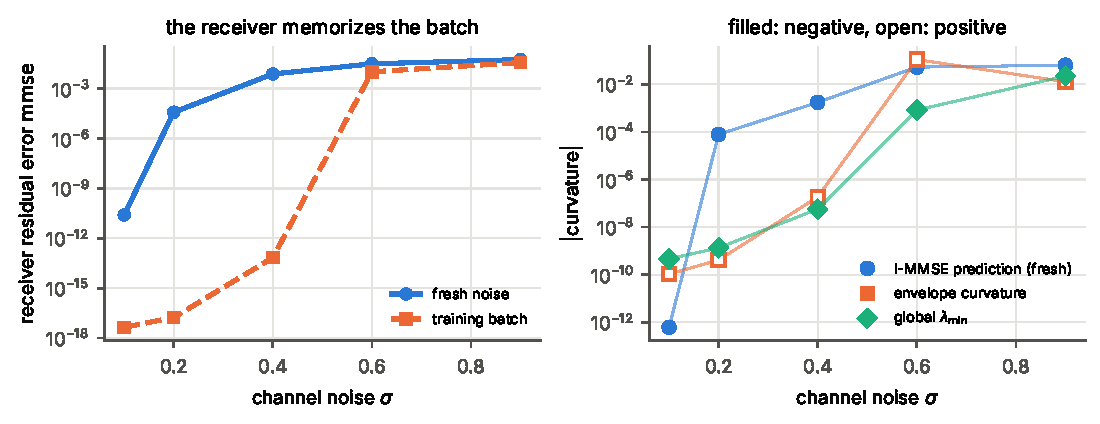
\includegraphics[width=0.9\linewidth]{figs/e13_saddle.pdf}
\caption{E13. Left: residual error of the polished receiver on its training batch and on fresh channel noise; for
$\sigma\le0.4$ the receiver has memorized the noise in its batch. Right: magnitudes of the I-MMSE prediction (with the
fresh-noise error), of the measured envelope curvature (median over features), and of the global smallest Hessian
eigenvalue; filled markers are negative, open markers positive.}
\label{fig:e13}
\end{figure}
Three findings, one of them negative.

\emph{At the operating point the legible code is flat, not a saddle.} At $\sigma=0.1$, the noise level of E10 and
E11, the polished point is critical to $6\times10^{-9}$, and the global $\lambda_{\min}$, the leak curvatures and the
envelope curvatures are all below $10^{-9}$ in magnitude. This is not an artefact. The
receiver's error on fresh noise is itself a few times $10^{-11}$, so \cref{prop:immse} predicts a negative curvature of
order $10^{-12}$. Every second derivative of the cross-entropy carries a factor of the receiver's residual error, and
a receiver that decodes almost perfectly sits on a plateau. There is no saddle to escape. Gradient descent has
nothing to follow, while Adam turns vanishing gradients into steps of size $\eta$. This is the second mechanism of
\cref{sec:saddle}, and it is the one that accounts for E11 at $d=12$: Adam on the sender spreads the code, the
spread buys nothing on the task, and SGD on the sender leaves the code where it is.

\emph{The receiver does not ignore empty coordinates.} \Cref{lem:stationary} assumes that the receiver puts no weight
on a coordinate that carries only noise. Trained receivers do: the weight on the empty coordinate we analyse is
comparable to the weight on owned coordinates at every $\sigma$ (\file{e13\_fresh.py}). Its cost is
second order in $\sigma$ and suppressed by the receiver's confidence, so it survives from initialization. The lemma
therefore holds only in a weaker form: the leak gradient is proportional to that weight times the residual error,
which is negligible at the operating point (E15, $d=12$) but not at high noise.

\emph{The quantitative curvature theory is not confirmed.} At $\sigma=0.2$ and $0.4$ everything is again flat, but
for a different reason: on its fixed batch the receiver has memorized the channel noise (residual error $10^{-17}$ and
$10^{-13}$ on the batch, against $4\times10^{-5}$ and $8\times10^{-3}$ on fresh noise). The Hessian we compute is the
Hessian of an overfit empirical loss, and the I-MMSE prediction with the fresh-noise error ($-8\times10^{-5}$,
$-2\times10^{-3}$) is orders of magnitude larger than anything measured. At $\sigma=0.6$ and $0.9$ the batch and
fresh errors are closer, and negative curvature appears: the global $\lambda_{\min}$ is $-8\times10^{-4}$ and
$-2\times10^{-2}$, and at $\sigma=0.9$ its eigenvector lies 85\% on leaks into empty coordinates. So the legible code
is a saddle at high noise. But it is not the saddle of \cref{sec:saddle}. The point is not critical in leak
directions (gradient about $2\times10^{-2}$, against $1.5$--$2.5\times10^{-3}$ within the support), the leak curvature is positive rather
than zero because the receiver reads the empty coordinate, and the per-feature envelope curvature is positive (for 23 of the 24
features) where \cref{prop:immse} predicts it negative. A clean test of the I-MMSE formula for trained receivers needs the Hessian of
the population loss (fresh noise and much larger batches), which we have not done.


\section{What this means for monitoring}\label{sec:monitoring}

We summarize what the toy model supports, what it does not, and what would test it at scale.

\emph{Supported.}
\begin{enumerate}[leftmargin=*, itemsep=2pt]
\item \emph{Frozen monitors decay; most of the decay is cheap to repair.} Removing a legibility pressure lets the
code move, and a frozen linear monitor loses about $0.2$ F1. Recalibrating a scale and bias per feature, with fresh
labels, recovers most of it. A monitor of a channel under training should be recalibrated on a schedule, not
frozen.
\item \emph{Where the public frame has spare capacity, the update rule of the writer decides legibility.} Plain SGD
on the parameters that write the message keeps features on their coordinates at no cost to the task, even with Adam
elsewhere. The mechanism is that near a well-trained legible code the loss is flat (E13), and Adam normalizes the
resulting tiny and noisy gradients into finite steps.
\item \emph{Legibility can be bought, at a price.} An $\ell_1$ budget in the public frame holds the code legible under
pressure and costs task performance.
\end{enumerate}

\emph{Not supported, or not tested.}
\begin{enumerate}[leftmargin=*, itemsep=2pt]
\item \emph{Spontaneous obfuscation under monitor pressure.} Putting a frozen monitor in the loss did not open a gap
between what the receiver uses and what a refit linear monitor reads. Obfuscation under monitor pressure has been
observed in reinforcement learning on chain-of-thought with large models~\cite{Baker}; this toy is too small and
too linear to say anything about that.
\item \emph{Optimizer control in superposition.} When the frame has no spare capacity, drift is first-order (E15),
and we found no update rule that both keeps the receiver improving and keeps the code legible.
\item \emph{The curvature theory.} The I-MMSE formula for the curvature at the legible code is proved for a Bayes
receiver and untested for trained ones (E13).
\item \emph{Anything at scale.} All of Part II is a 16-dimensional channel.
\end{enumerate}

\emph{The reassuring disanalogy.} No-cloning has no classical counterpart (\S\ref{sec:dictionary}). Whatever
obstructs a monitor from reading a classical channel is ignorance of the code or the cost of decoding, never a law of
nature. Every effect in Part II was visible to a monitor that was allowed to refit.

\subsection*{Predictions for latent-reasoning models}
The natural test bed is continuous chain-of-thought~\cite{Coconut}: a model feeds its own hidden state back as the
next input, so it is simultaneously the sender and the receiver of an activation-space message. Starting from a
text-CoT checkpoint (legible by construction in the vocabulary frame, or in a sparse-autoencoder frame), the notes
make these predictions.
\begin{prediction}
Logit-lens and SAE-frame legibility of the latent thoughts decays when the text bottleneck is removed, and the
decay is mostly recoverable by recalibrating a frozen probe (E10 at scale).
\end{prediction}
\begin{prediction}
If the frame has spare capacity (features the message is not yet using), training the parameters that write the
latent thought with plain SGD, and everything else with AdamW, slows the spread of the message relative to AdamW
everywhere, at matched task accuracy. If the frame is saturated, it does not (E11 at scale).
\end{prediction}
\begin{prediction}
Near a well-trained legible checkpoint with spare frame capacity, the expected gradient of the writer's parameters
in directions that leave the frame is close to zero, while AdamW's update along those directions is as large as
along any other (E13 and E15 at scale).
\end{prediction}
These need a model of about $10^8$ parameters and tens of GPU-hours; none has been run.

\section{Status ledger}\label{sec:ledger}
\begin{center}\small
\begin{tabularx}{\linewidth}{@{}>{\raggedright\arraybackslash}X l l@{}}\toprule
claim & status & where \\\midrule
Random codes over $\R$ and $\C$ are isometries on sets with $\log\abs\Sigma\ll\beta N\delta^2$ & proved & \cref{thm:main} \\
AEHPV low-complexity isometry and RIP are two cases of it & proved & \cref{cor:aehpv,cor:rip} \\
Exact overlap variances; real/complex difference is the $\Omega$ Brauer term & proved, checked & \cref{prop:variances}, E01 \\
Any unit-norm tight frame matches Haar at second order & proved & \cref{prop:frame-identity} \\
State-independent reconstruction is biased by $\approx e^{-S_{\rm BH}}\tr A$ & proved & \cref{prop:statedep} \\
Page $\leftrightarrow$ Donoho--Tanner; QES crossover $\leftrightarrow$ ALMT edge & proved (each side), structural analogy & \S\ref{sec:page} \\
Python's lunch $\leftrightarrow$ computational--statistical gap & analogy (hardness conjectural) & \S\ref{sec:page} \\
Trained toy codes are tight, Haar at 2nd order, better than Haar at the extremes & checked & E02 \\
Language-model embeddings: anisotropic, heavy-tailed, Haar-like recovery & checked & E03 \\
Legible codes are critical in leaks to empty coordinates (if the receiver ignores them) & proved & \cref{lem:stationary} \\
\ldots\ and, from E11's starting codes, critical at $d=12$ but not at $d=32$ & checked & E15 \\
Envelope curvature $=-\phi'^2\mmse/\sigma^2$ for the Bayes receiver & proved & \cref{prop:immse} \\
\ldots\ and for trained receivers & not confirmed & E13 \\
At the operating noise the legible code is flat ($\abs{\lambda}<10^{-9}$) & checked & E13 \\
Gradient descent escapes in $\sim\log(1/z_0)/\eta\abs{\lambda_-}$, Adam in $O(1)$ & heuristic; checked in isolation & E14 \\
Writer's update rule controls spread when the frame has spare capacity & checked & E11, $d=12$ \\
\ldots\ and not in superposition & checked (negative) & E11, $d=32$ \\
Monitor in the loss grows a hidden channel & not supported at this scale & E10 \\
Anything about large models & untested; predictions only & \S\ref{sec:monitoring} \\
\bottomrule\end{tabularx}
\end{center}
